\documentclass{beamer}
\usepackage[utf8]{inputenc}
\usetheme{Pittsburgh}
\usepackage{graphicx}

\title{EU-projekt TG4NP \\Tourist Guide for Northen Periphery}
\author{Emil Norgberg Strömgren \\ Rickard Nordlander \\ Niil Öhlin}
\date{\today}
\begin{document}
	\begin{frame}
		\titlepage
	\end{frame}
	
	\begin{frame}{Personer}
		\begin{columns}
			\begin{column}[T]{5cm}
				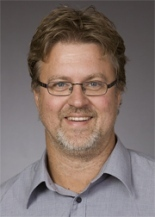
\includegraphics[scale=0.7]{furberg_lars2.jpg}
			\end{column}
			\begin{column}[T]{5cm}
				\begin{itemize}
					\item Lars Furberg
					\item<2-> Fyra personer
					\item<3-> Administrativa roller
					\item<4-> Studenter
					\item<5-> University of Ulster. Irland
					\item<6-> Turistföretag
					\item<7-> Skellefteå kommun
				\end{itemize}
			\end{column}

		\end{columns}
	\end{frame}

	\begin{frame}{Syfte}
		Utveckla en mobilapplikation för att ge information till turister i norra europa
		\begin{itemize}
			\item<1-> Identifiera artefakter
			\item<2-> Utveckla ett återanvändbart ramverk
			\item<3-> Underlätta för turister
			\item<4-> Främja turismen i avlägsna platser
		\end{itemize}
	\end{frame}

	\begin{frame}{Tidigare landvinningar}
		Ganska ungt område.
	\end{frame}

	\begin{frame}{Genomförande}
		\begin{itemize}
			\item<1-> I sitt slutskede
			\item<2-> Tre timmar i veckan
			\item<3-> Tidigare veckovis heltid
			\item<4-> Konstant rapportering till lead partner
			\item<5-> Studenter som går mobila system i skellefteå
			\item<6-> Inga definierade förkunskaper
			\item<7-> Administration och finans av EU
			\item<8-> Påfrestande byrokrati
			\item<9-> Nätverkande. Trevliga människor
		\end{itemize}
	\end{frame}

	\begin{frame}{Konsekvensker}
		\begin{itemize}
			\item<1-> Tekniskt framåtskridande inom utveckling av mobila applikationer.
			\item<2-> Ökad omsättning för lokala företag
			\item<3-> Ökad internationalisering
		\end{itemize}
	\end{frame}

	\begin{frame}{Utmaningar}
		\begin{itemize}
			\item<1-> Stress
			\item<2-> Byrokrati 
			\item<3-> Försenade rapporter 
			\item<4-> Långtidssjukskrivningar
		\end{itemize}
	\end{frame}

	\begin{frame}{Avslutning}
		Projektet har lett till 
		\begin{itemize}[<+->]
			\item Framsteg i turistindustrin
			\item Ökad kunskap om användningen av mobila appar
			\item Ett koncept / ramverk om turisthantering via modern teknik
			\item Ökad mognad hos turistföretagen i arbetet bakom mobilutveckling
			\item Nätverkandet ger kontakter till framtida projekt
		\end{itemize}
	\end{frame}
\end{document}
